\RequirePackage{luatex85}
\documentclass[border=1pt]{standalone}
\usepackage{tikz}
\usetikzlibrary{shapes.geometric, arrows}

%%%%%%%%%%%%%%%%%%%%%%%%%%%%%%%%%%%%%%%%%%%%%%%%%%%%%%%%%%%%%%%%%%%%%%%%%%%%%%%%
%%%%%%%%%%%%%%%%%%%%                 colours                %%%%%%%%%%%%%%%%%%%% 
%%%%%%%%%%%%%%%%%%%%%%%%%%%%%%%%%%%%%%%%%%%%%%%%%%%%%%%%%%%%%%%%%%%%%%%%%%%%%%%%

\definecolor{tugreen}{RGB}{128, 186, 38}
\definecolor{tucitron}{RGB}{249, 219, 0}



%%%%%%%%%%%%%%%%%%%%%%%%%%%%%%%%%%%%%%%%%%%%%%%%%%%%%%%%%%%%%%%%%%%%%%%%%%%%%%%%
%%%%%%%%%%%%%%%%%%%%                 Boxes                  %%%%%%%%%%%%%%%%%%%% 
%%%%%%%%%%%%%%%%%%%%%%%%%%%%%%%%%%%%%%%%%%%%%%%%%%%%%%%%%%%%%%%%%%%%%%%%%%%%%%%%
\tikzstyle{normalBox} = [shape=rectangle, draw=black, text=black, thick, 	
	align=center, fill=white]

\tikzstyle{roundBox} = [shape=circle, draw=black, text=black, thick, 	
	align=center, fill=white]

\tikzstyle{alternBox} = [shape=rectangle, text=white, thick, align=center, 
	fill=black, rounded corners]


%%%%%%%%%%%%%%%%%%%%%%%%%%%%%%%%%%%%%%%%%%%%%%%%%%%%%%%%%%%%%%%%%%%%%%%%%%%%%%%%
%%%%%%%%%%%%%%%%%%%%                 Arrows                 %%%%%%%%%%%%%%%%%%%% 
%%%%%%%%%%%%%%%%%%%%%%%%%%%%%%%%%%%%%%%%%%%%%%%%%%%%%%%%%%%%%%%%%%%%%%%%%%%%%%%%

\tikzstyle{normalArrow} = [thick,->,>=stealth, draw=black]

\usepackage[utf8]{inputenc}
\usepackage[T1]{fontenc}
\usepackage[sfdefault]{FiraSans}


\tikzstyle{NormalBox} = [normalBox, text width =2.5cm, minimum height=1cm]
\tikzstyle{AlternBox} = [alternBox, text width =2.5cm, minimum height=1cm]

\begin{document}
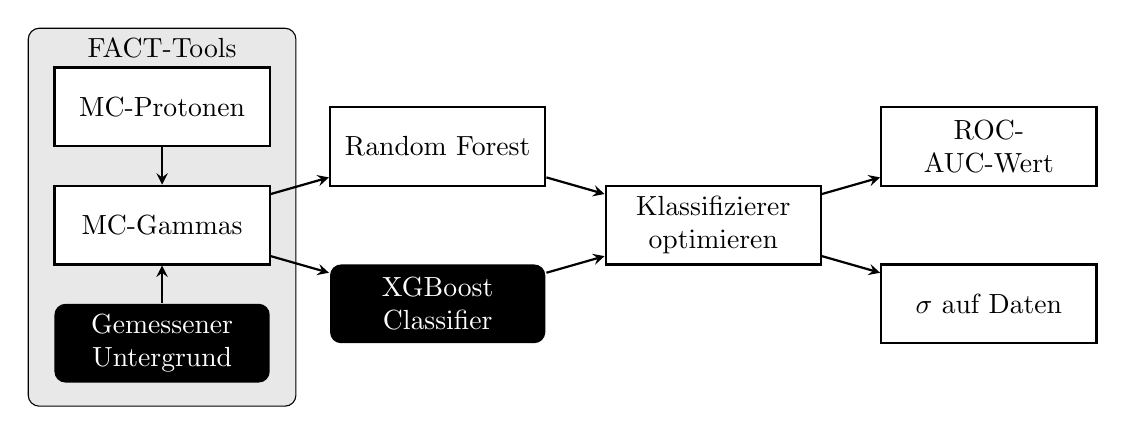
\begin{tikzpicture}[node distance=1.5cm]
  \draw [fill=black!09!white, draw=black, rounded corners] (-1.7,1) rectangle (1.7,-3.8);
  \draw (0,0.75) node[text=black] {FACT-Tools};
  \node (MCPRO) [NormalBox] {MC-Protonen};
  \node (MCGAM) [NormalBox, below of=MCPRO] {MC-Gammas};
  \node (MEPRO) [AlternBox, below of=MCGAM] {Gemessener Untergrund};
  \node (TREE) [NormalBox, right of=MCGAM, xshift=2cm, yshift=1cm] {Random Forest};
  \node (XGBC) [AlternBox, right of=MCGAM, xshift=2cm, yshift=-1cm] {XGBoost Classifier};
  \node (OPTI) [NormalBox, right of=TREE, xshift=2cm, yshift=-1cm] {Klassifizierer optimieren};
  \node (ROC) [NormalBox, right of=OPTI, xshift=2cm, yshift=1cm] {ROC-AUC-Wert};
  \node (SIGMA) [NormalBox, right of=OPTI, xshift=2cm, yshift=-1cm] {$\sigma$ auf Daten};

  \draw [normalArrow] (MCPRO) -- (MCGAM);
  \draw [normalArrow] (MEPRO) -- (MCGAM);
  \draw [normalArrow] (MCGAM) -- (TREE);
  \draw [normalArrow] (MCGAM) -- (XGBC);
  \draw [normalArrow] (TREE) -- (OPTI);
  \draw [normalArrow] (XGBC) -- (OPTI);
  \draw [normalArrow] (OPTI) -- (ROC);
  \draw [normalArrow] (OPTI) -- (SIGMA);


\end{tikzpicture}
\end{document}
